\documentclass[12pt,a4paper]{article}

% --- packages ---
\usepackage[top=2.5cm, bottom=2.5cm, left=2.8cm, right=2.8cm]{geometry}
\usepackage{graphicx}
\usepackage{subcaption}
\usepackage{amsmath}
\usepackage{booktabs}
\usepackage{hyperref}
\usepackage{xcolor}
\usepackage{setspace}
\usepackage{parskip}
\usepackage{titlesec}
\usepackage{fancyhdr}
\usepackage{float}
\usepackage[numbers,sort&compress]{natbib}

\hypersetup{
    colorlinks=true,
    linkcolor=black,
    citecolor=black,
    urlcolor=blue
}

\graphicspath{{results/figures/}}

\pagestyle{fancy}
\fancyhf{}
\rhead{Complex Networks -- Final Project}
\lhead{Reihaneh Hasani}
\rfoot{\thepage}

\titleformat{\section}{\large\bfseries}{}{0em}{\thesection.\quad}
\titleformat{\subsection}{\normalsize\bfseries}{}{0em}{\thesubsection\quad}

\onehalfspacing

% ============================================================
\begin{document}

% --- title page ---
\begin{titlepage}
    \centering
    \vspace*{2cm}

    {\LARGE\bfseries Automatic Analysis of Scientific Literature\\[0.4em]
    on Antimicrobial Resistance:\\[0.4em]
    Citation Network, Communities, and\\[0.4em]
    Temporal Evolution of Research Topics\par}

    \vspace{1.5cm}
    {\large\itshape Reihaneh Hasani\par}
    \vspace{0.5cm}
    {\normalsize Complex Networks\par}
    \vspace{0.3cm}
    {\normalsize \today\par}

    \vspace{2cm}

    \begin{abstract}
    \noindent
    This report presents a network-based analysis of the scientific literature on
    Antimicrobial Resistance (AMR), constructed from PubMed citation data.
    The dataset comprises 235\,871 papers and 524\,482 citation links spanning
    the years 1965 to 2023.
    I built a directed citation graph and applied the Louvain community detection
    algorithm to identify clusters of related research topics.
    The partition yields 30\,086 communities with a modularity of 0.746,
    and the ten largest communities together account for more than 120\,000 papers.
    To characterise each community thematically, I applied TF-IDF analysis over
    the abstracts and MeSH descriptors of member papers.
    The results reveal clearly separated research fields, including environmental AMR
    and the One Health framework, efflux-pump-mediated resistance in Gram-negative
    bacteria, plasmid genetics and horizontal gene transfer, antifungal resistance,
    and tuberculosis.
    A temporal analysis over 5-year windows shows that environmental AMR has grown
    from a marginal topic before 2005 into the most internally connected community
    in the 2020--2023 period, while the foundational genetics community dominated
    the literature in the 1970s.
    \end{abstract}
\end{titlepage}

\tableofcontents
\newpage

% ============================================================
\section{Introduction}

Antimicrobial resistance (AMR) is one of the most pressing threats to global public health.
The World Health Organization has classified AMR as a top-ten global health threat,
and projections suggest it could cause 10 million deaths annually by 2050 if left unchecked
\cite{who_amr_2015}.
The scientific response to this crisis has been enormous: tens of thousands of papers are
published each year across disciplines that range from molecular microbiology to
environmental engineering and health policy.

Navigating this body of literature is itself a complex problem.
Network analysis of citation data provides a principled way to map the intellectual
landscape of a research field: papers that cite each other frequently tend to cluster
together, and those clusters correspond to coherent research communities sharing methods,
organisms, and concepts.
By applying community detection and text-mining techniques to a large citation network,
it is possible to identify the main sub-disciplines, rank papers by structural
importance, and track how the relative prominence of each topic has evolved over time.

This project analyses a citation network derived from PubMed, containing papers
retrieved through the MeSH descriptor \textit{Drug Resistance, Microbial} together
with all the papers they cite.
The main goals are:
\begin{enumerate}
    \item Construct and characterise the AMR citation network as a graph.
    \item Detect communities corresponding to distinct research topics.
    \item Automatically label each community using TF-IDF text analysis.
    \item Study the temporal evolution of community size and centrality.
\end{enumerate}

% ============================================================
\section{Dataset}

\subsection{Source and Construction}

The dataset was provided as two CSV files exported from PubMed/MEDLINE.
The \textit{nodes} file contains one row per paper with the following attributes:
PubMed ID (PMID), article title, journal, year of publication, MeSH descriptors,
author keywords, abstract text, and a boolean flag \texttt{on\_topic}.
The \textit{edges} file contains one row per citation, recording the PMID of the citing
paper and the PMID of the cited paper.

Papers were collected in two stages.
First, all papers indexed with the MeSH descriptor \emph{Drug Resistance, Microbial}
were retrieved (\texttt{on\_topic = True}).
Second, any paper cited by an on-topic paper but not itself retrieved in the first stage
was added to the dataset (\texttt{on\_topic = False}) to ensure that the citation
network is internally connected and that foundational references are not lost.

\subsection{Basic Statistics}

After loading and cleaning the data (parsing list-valued columns, handling missing years,
and removing edges whose endpoints fall outside the node set), the working dataset
contains:

\begin{table}[H]
\centering
\caption{Dataset overview.}
\begin{tabular}{lr}
\toprule
\textbf{Property} & \textbf{Value} \\
\midrule
Total papers (nodes)       & 235\,871 \\
On-topic papers            & 61\,536  \\
Cited-only papers          & 174\,335 \\
Citation links (edges)     & 524\,482 \\
Year range                 & 1965--2023 \\
\bottomrule
\end{tabular}
\label{tab:dataset}
\end{table}

The difference between the 1\,019\,656 raw edges in the original file and the 524\,482
retained edges is due to citations that point to papers outside the node set (i.e.,
papers that were never retrieved in either collection stage).

% ============================================================
\section{Methodology}

\subsection{Network Construction}

I represent the literature as a \textit{directed} graph $G = (V, E)$, where each node
$v \in V$ is a paper identified by its PMID, and each directed edge $(u, v) \in E$
indicates that paper $u$ cites paper $v$.
The direction encodes the temporal and intellectual dependency: a citing paper builds
upon the knowledge of the cited one.

The graph was built using the \texttt{python-igraph} library \cite{igraph2006}, which
offers efficient implementations of both graph construction and community detection.
Rather than the NetworkX $\to$ GraphML $\to$ igraph route (which is prohibitively slow
for graphs of this size), I mapped the edge list directly to igraph vertex indices using
vectorised pandas operations.

Table~\ref{tab:graph} summarises the main properties of the resulting graph.
The low density ($\approx 9.4 \times 10^{-6}$) and the large number of weakly connected
components (29\,994) are both expected for a citation network: many papers cite only a
handful of others, and not all cited papers are reachable from one another.

\begin{table}[H]
\centering
\caption{Properties of the directed citation graph.}
\begin{tabular}{lr}
\toprule
\textbf{Property} & \textbf{Value} \\
\midrule
Nodes                         & 235\,871 \\
Edges                         & 524\,482 \\
Density                       & $9.4 \times 10^{-6}$ \\
Average degree (undirected)   & 4.45 \\
Weakly connected components   & 29\,994 \\
\bottomrule
\end{tabular}
\label{tab:graph}
\end{table}

\subsection{Community Detection}

Community detection was performed on the \textit{undirected} version of the graph,
as required by the algorithms used.
I applied the \textbf{Louvain algorithm} (also called \texttt{community\_multilevel} in
igraph) \cite{blondel2008}, which optimises modularity by iteratively merging nodes and
communities in two phases.
This method scales well to graphs with millions of edges and reliably produces
high-modularity partitions.

For comparison, the leading-eigenvector method \cite{newman2006} was also implemented
but is better suited to smaller subgraphs due to its $O(|V|^2)$ memory requirements.

Modularity $Q$ measures the quality of a partition and is defined as:
\begin{equation}
Q = \frac{1}{2m} \sum_{i,j} \left[ A_{ij} - \frac{k_i k_j}{2m} \right] \delta(c_i, c_j)
\end{equation}
where $A$ is the adjacency matrix, $k_i$ is the degree of node $i$, $m$ is the total
number of edges, and $\delta(c_i, c_j) = 1$ if nodes $i$ and $j$ belong to the same
community \cite{fortunato2010}.

\subsection{Topic Profiling via TF-IDF}

To automatically label each community with its research topic, I concatenated the
abstract texts, MeSH descriptors, and author keywords of all papers belonging to that
community into a single document.
I then fitted a TF-IDF (Term Frequency -- Inverse Document Frequency) model
\cite{salton1988} treating each community as one document.

The TF-IDF score of term $t$ in community $c$ is:
\begin{equation}
\mathrm{TFIDF}(t, c) = \mathrm{TF}(t,c) \cdot \log\left(\frac{N}{|\{c' : t \in c'\}|}\right)
\end{equation}
where $N$ is the total number of communities and $\mathrm{TF}(t,c)$ uses sublinear
scaling ($\log(1 + \mathrm{count})$).
Terms with high TF-IDF scores are distinctive for a community, meaning they appear
frequently in its papers but rarely in papers from other communities.
Only communities with at least 20 papers were included in the model;
communities smaller than this threshold are mostly isolated papers with insufficient
text to produce reliable results.

\subsection{Temporal Analysis}

To study the evolution of the field over time, I divided the dataset into 5-year windows
(1965--1969, 1970--1974, \ldots, 2020--2023) and built a separate subgraph for each
window containing only the papers published in that period and the citations between them.
This \textit{windowed} approach (as opposed to a cumulative growing-network approach)
highlights the internal activity of each time period independently.

For each temporal subgraph I computed three centrality measures aggregated by community:
\begin{itemize}
    \item \textbf{Average degree}: average number of connections per paper within the window.
    \item \textbf{Average betweenness centrality}: fraction of shortest paths passing
          through each node (approximated by vertex sampling for speed).
    \item \textbf{Average PageRank}: stationary probability of a random walker
          reaching each node.
\end{itemize}
These metrics jointly capture how prominent and interconnected each community was during
each period.

% ============================================================
\section{Results}

\subsection{Network Topology}

The degree distribution of the AMR citation network follows a heavy tail, as is typical
of citation networks: most papers have few citations while a small number are cited
thousands of times.
The average degree over the undirected graph is 4.45.
The most connected paper in the entire network is
\textit{``The challenge of efflux-mediated antibiotic resistance in Gram-negative
bacteria''} (2015), with a total degree of 1\,176, meaning it is connected to 1\,176
other papers in the dataset either as a citing or cited paper.

The large number of weakly connected components (29\,994) reflects the many papers in the
dataset that were cited only once or twice by an on-topic paper and are not connected to
the main body of the network.
The largest weakly connected component contains the vast majority of on-topic papers.

\subsection{Community Structure}

\begin{figure}[H]
    \centering
    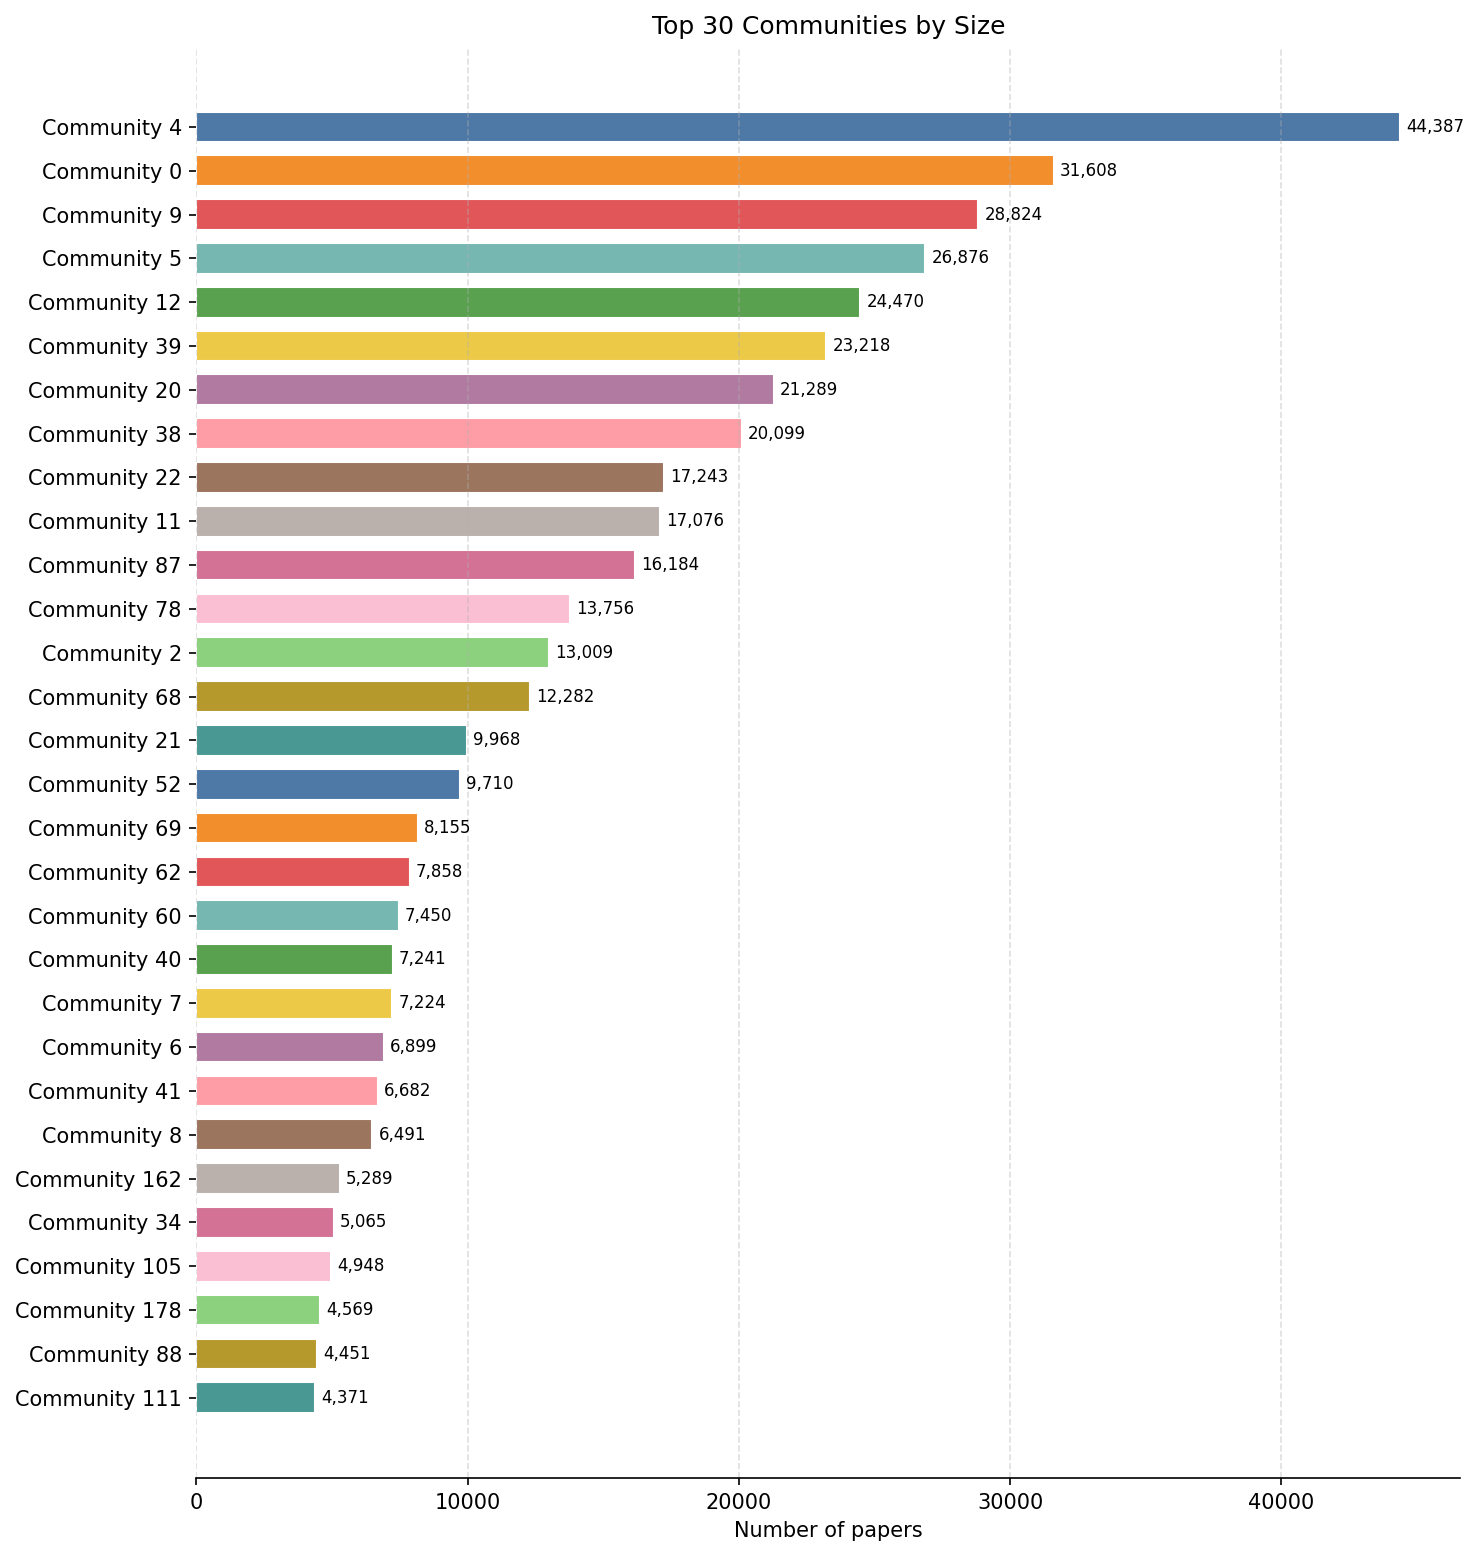
\includegraphics[width=\textwidth]{community_sizes.png}
    \caption{Top 30 communities by number of papers. The four largest communities
             each contain between 16\,000 and 18\,000 papers, reflecting the
             roughly equal prominence of the main AMR research pillars.}
    \label{fig:sizes}
\end{figure}

The Louvain algorithm identified \textbf{30\,086 communities} with a modularity of
\textbf{$Q = 0.746$}.
This is a high modularity value, indicating that papers within communities are much more
densely cited among themselves than would be expected by chance.

As shown in Figure~\ref{fig:sizes}, the size distribution has a heavy tail.
The four largest communities (C65, C8, C2, C102) each contain between 16\,000 and
18\,000 papers, forming the dominant pillars of AMR research.
Below them, community sizes decrease steeply, and the majority of the 30\,086 communities
consist of fewer than 10 papers (isolated citation clusters).

Table~\ref{tab:communities} summarises the ten largest communities.
The median year of publication is a useful proxy for when each community was most active:
C102 (foundational genetics) has a median year of 1981, while C65 (environmental AMR)
has a median of 2015, reflecting its emergence as a research priority only in the past
two decades.

\begin{table}[H]
\centering
\caption{The ten largest communities. ``On-topic'' counts papers retrieved via the
         \emph{Drug Resistance, Microbial} descriptor. Density is computed within
         each community subgraph.}
\begin{tabular}{rrrrrll}
\toprule
\textbf{ID} & \textbf{Size} & \textbf{On-topic} & \textbf{Density} &
\textbf{Med.\ Year} & \textbf{Main topic} \\
\midrule
C65  & 18\,067 & 2\,400 & $2.4 \times 10^{-4}$ & 2015 & Environmental AMR / One Health \\
C8   & 16\,580 & 2\,340 & $2.3 \times 10^{-4}$ & 2011 & Global AMR mechanisms \& policy \\
C2   & 16\,330 & 2\,857 & $3.8 \times 10^{-4}$ & 2000 & Efflux pumps, Gram-negatives \\
C102 & 15\,985 & 2\,644 & $3.0 \times 10^{-4}$ & 1981 & Plasmid genetics, HGT \\
C37  & 11\,597 & 1\,487 & $3.5 \times 10^{-4}$ & 1992 & Antifungal resistance \\
C4   & 10\,446 & 2\,549 & $5.7 \times 10^{-4}$ & 1995 & Gram-positives (MRSA, VRE) \\
C0   & 10\,028 & 2\,357 & $4.8 \times 10^{-4}$ & 1991 & Beta-lactamases \\
C36  &  8\,287 & 1\,614 & $4.7 \times 10^{-4}$ & 1996 & Mycobacterium tuberculosis \\
C18  &  7\,737 & 1\,431 & $5.8 \times 10^{-4}$ & 1997 & Ribosome-targeting antibiotics \\
C5   &  7\,034 & 1\,629 & $6.3 \times 10^{-4}$ & 1997 & Lateral gene transfer, trimethoprim \\
\bottomrule
\end{tabular}
\label{tab:communities}
\end{table}

\begin{figure}[H]
    \centering
    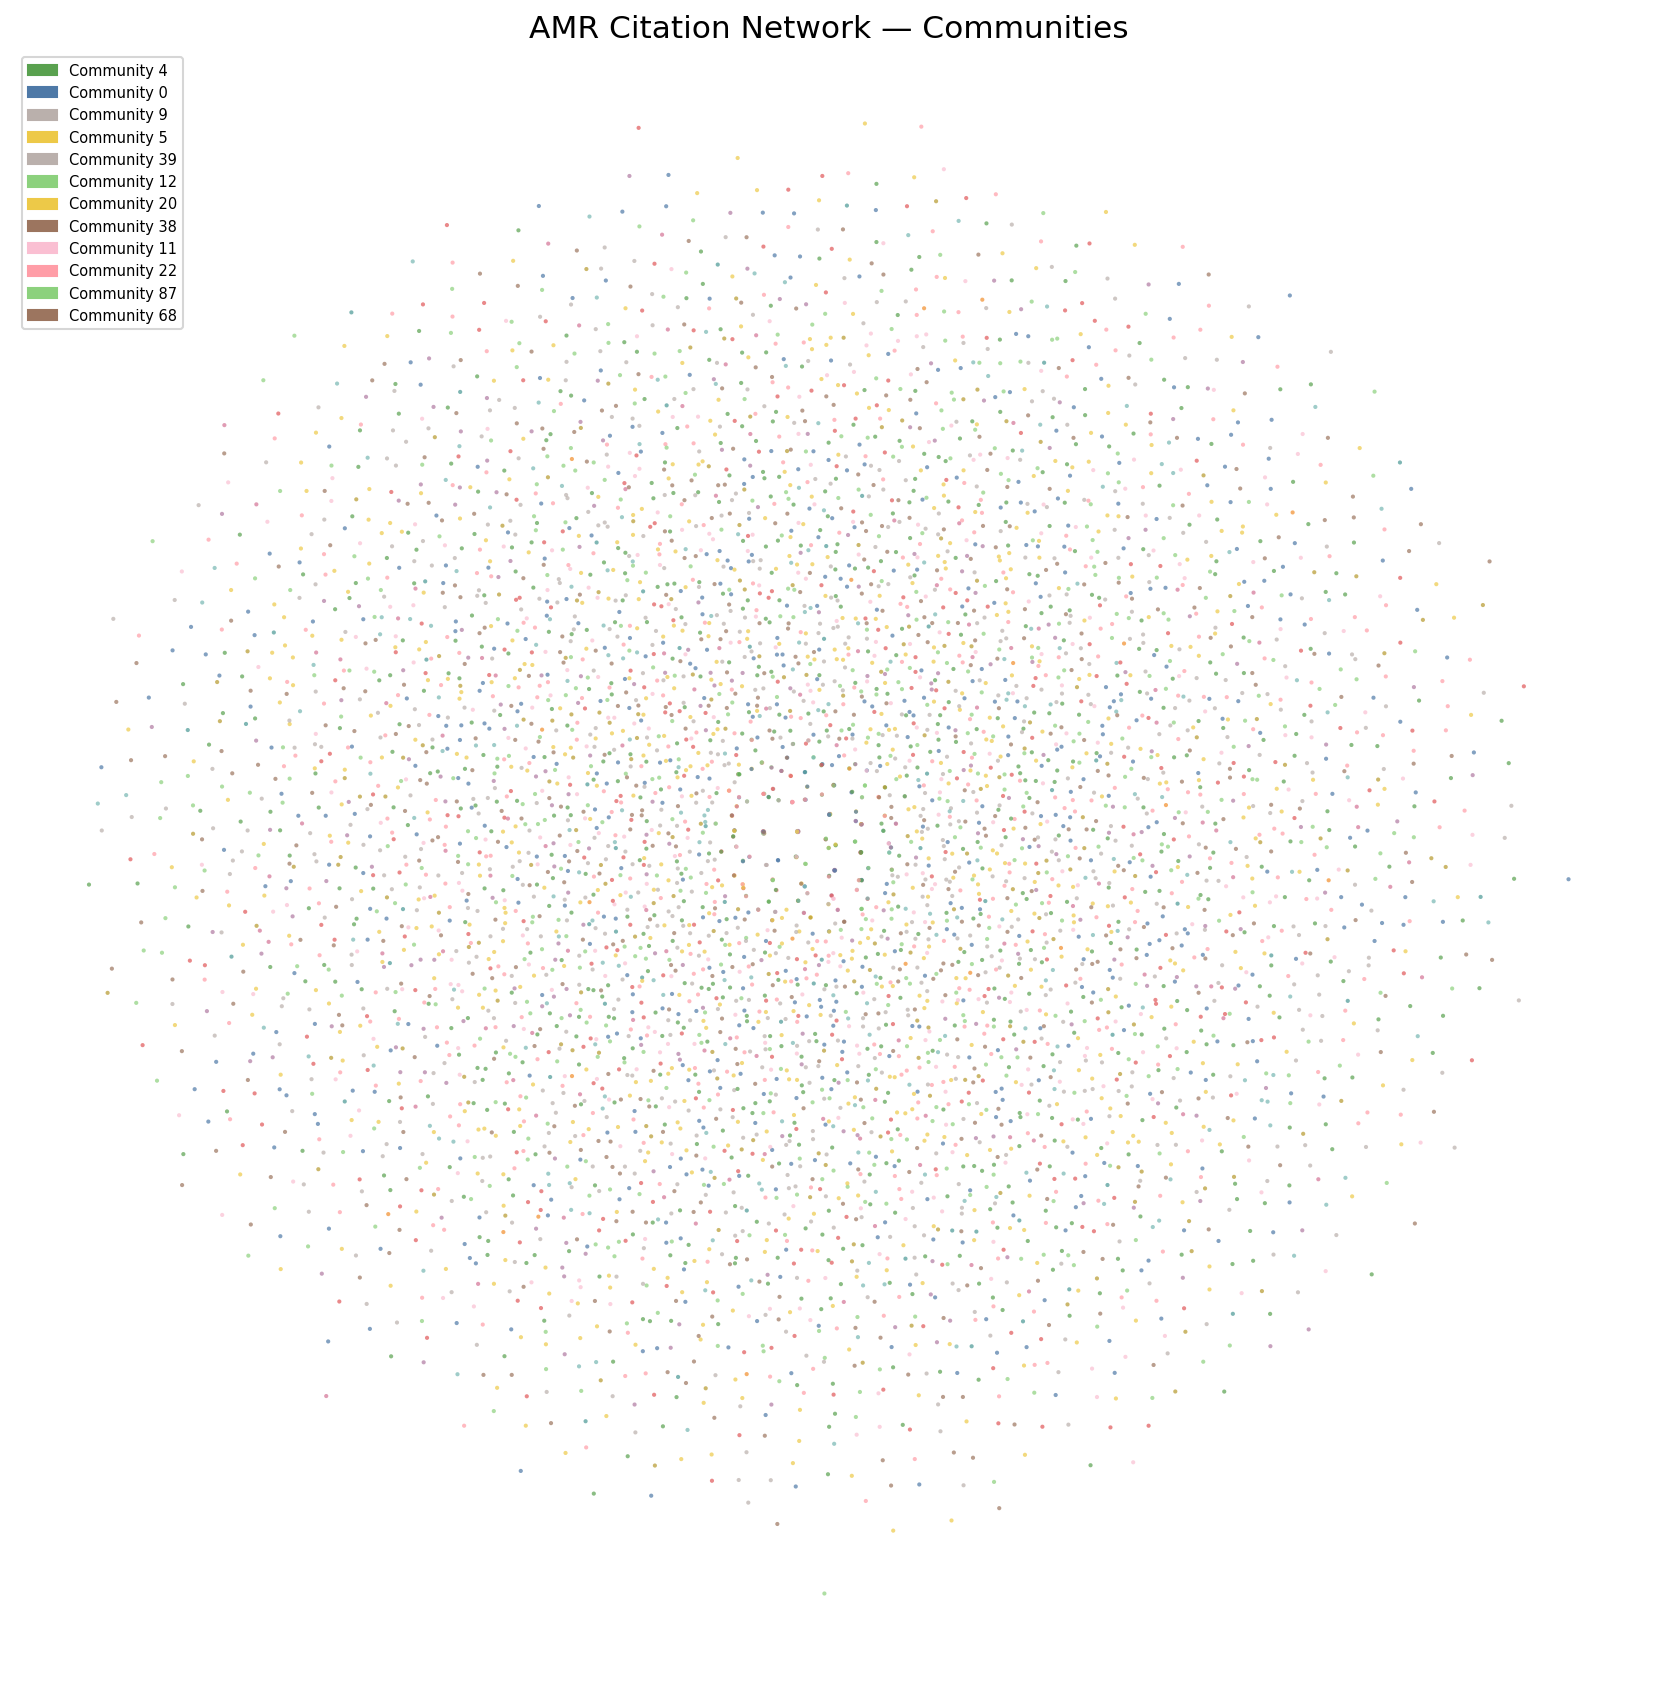
\includegraphics[width=\textwidth]{network_layout.png}
    \caption{Visualisation of the citation network (6\,000 randomly sampled nodes)
             using the DrL large-graph layout algorithm \cite{martin2011}.
             Colours indicate community membership.
             The spatial separation of colour clusters confirms that the Louvain
             partition recovers structurally coherent groups.}
    \label{fig:layout}
\end{figure}

\subsection{Topic Profiling}

\subsubsection{Community 65 -- Environmental AMR and One Health}

Community C65 is the largest community (18\,067 papers) and the most recent in terms of
median publication year (2015).
Its TF-IDF top terms include: \textit{args} (antibiotic resistance genes),
\textit{wwtps} (wastewater treatment plants), \textit{sewage sludge}, \textit{wwtp},
\textit{wastewater}, \textit{composting}, \textit{manure}, \textit{mges} (mobile
genetic elements), and \textit{arb} (antibiotic-resistant bacteria).

These terms precisely characterise the \textbf{environmental AMR} field, which studies
the dissemination of resistance genes through environmental compartments (water, soil,
agricultural waste) and their transfer into clinical settings via the One Health
framework \cite{onehealth}.
The word cloud in Figure~\ref{fig:wc_c65} confirms this interpretation, prominently
featuring \textit{gene}, \textit{resistance}, \textit{water}, \textit{soil},
\textit{microbiome}, \textit{plasmid}, and \textit{environmental}.

\begin{figure}[H]
    \centering
    \begin{subfigure}[b]{0.95\textwidth}
        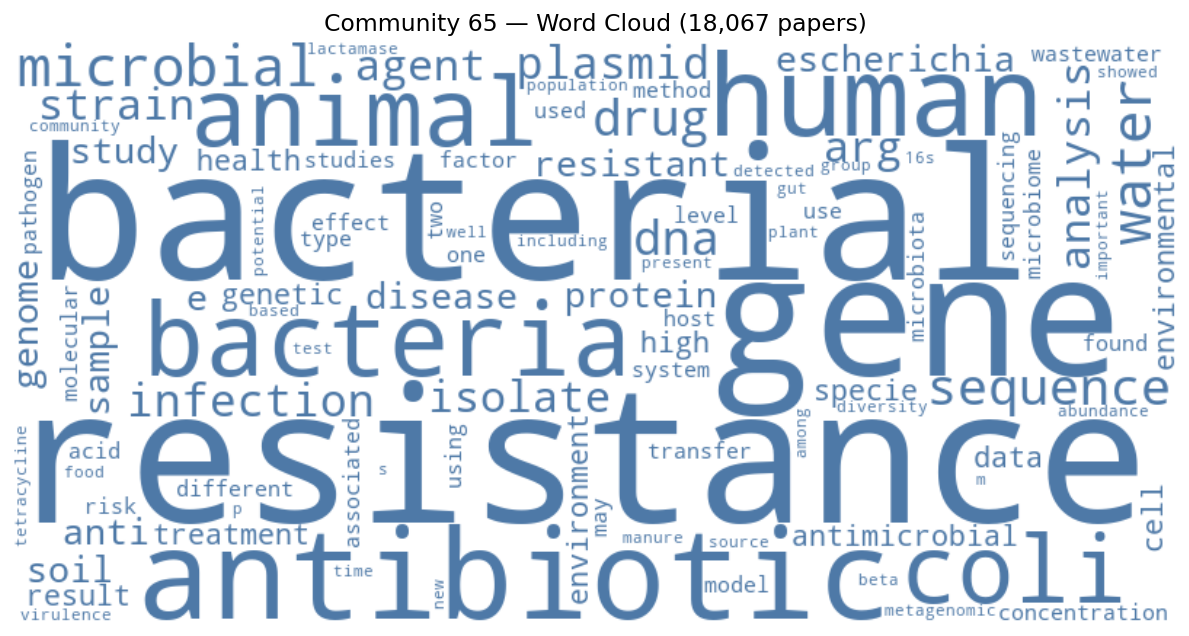
\includegraphics[width=\textwidth]{wordcloud_c65.png}
        \caption{Community C65 -- Environmental AMR / One Health (18\,067 papers).}
        \label{fig:wc_c65}
    \end{subfigure}
    \vspace{0.5em}

    \begin{subfigure}[b]{0.95\textwidth}
        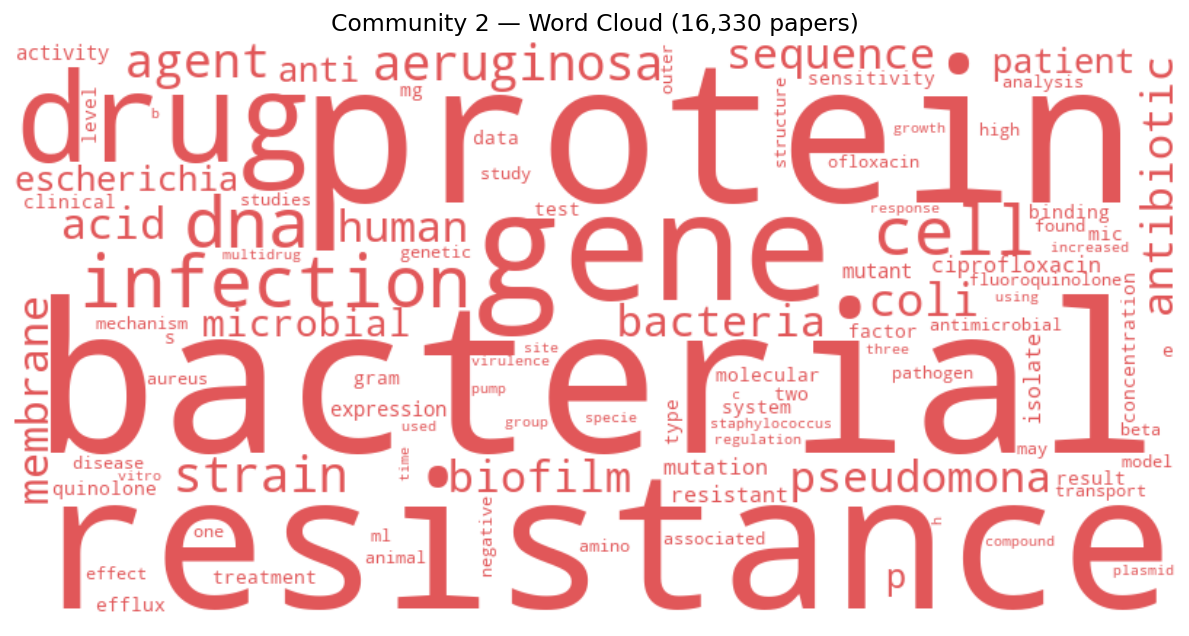
\includegraphics[width=\textwidth]{wordcloud_c2.png}
        \caption{Community C2 -- Efflux pumps / Gram-negative resistance (16\,330 papers).}
        \label{fig:wc_c2}
    \end{subfigure}
    \caption{Word clouds generated from the aggregated text (abstracts + MeSH descriptors)
             of papers in each community. Word size is proportional to frequency.}
    \label{fig:wordclouds}
\end{figure}

\subsubsection{Community 2 -- Efflux Pumps and Gram-Negative Resistance}

Community C2 (16\,330 papers) groups together research on the molecular mechanisms of
efflux-mediated resistance in Gram-negative bacteria.
Its top TF-IDF terms are: \textit{oprm}, \textit{mexab}, \textit{acrb}, \textit{nora},
\textit{soxs}, \textit{lasr}, \textit{fleroxacin}, \textit{oprd}, \textit{acrab},
\textit{rnd}, \textit{trovafloxacin}, \textit{persisters}, \textit{cftr},
\textit{pseudomallei}, \textit{tolc}.

These terms refer directly to the two canonical RND-type efflux pump systems:
\textbf{MexAB-OprM} in \textit{Pseudomonas aeruginosa} and \textbf{AcrAB-TolC} in
\textit{Escherichia coli}.
Both systems extrude a wide range of antibiotics, including fluoroquinolones (fleroxacin,
trovafloxacin), and are major contributors to clinical multidrug resistance.
The term \textit{persisters} reflects the growing understanding that efflux pumps also
play a role in antibiotic tolerance and persister cell formation \cite{blair2015}.
The TF-IDF bar chart and word cloud for this community are shown in
Figures~\ref{fig:tfidf} and~\ref{fig:wordclouds}(b).

\begin{figure}[H]
    \centering
    \begin{subfigure}[b]{0.95\textwidth}
        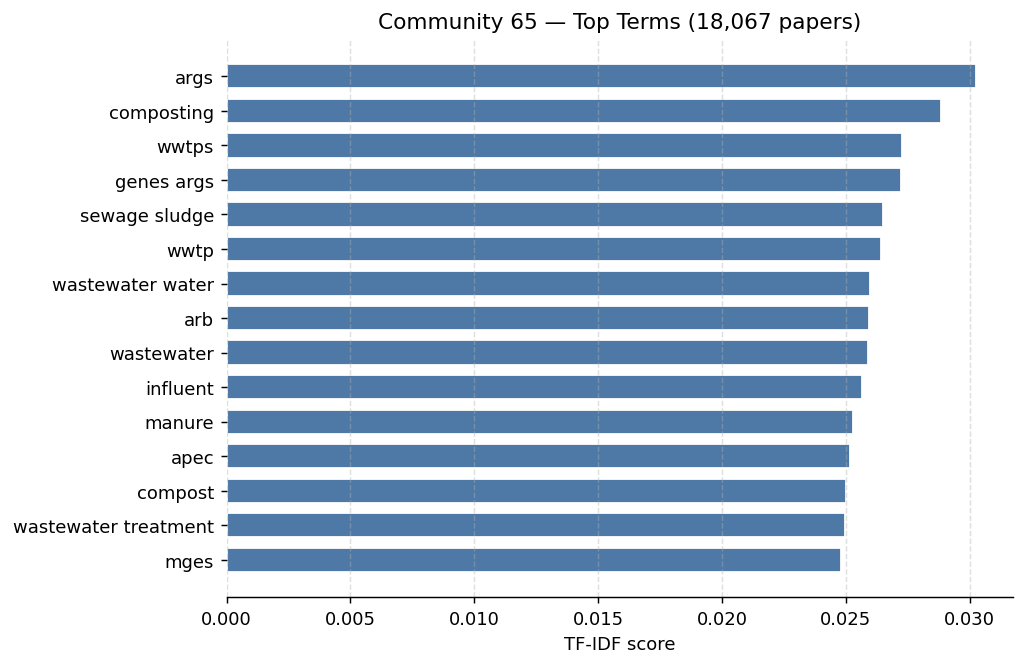
\includegraphics[width=\textwidth]{top_terms_c65.png}
        \caption{Top TF-IDF terms for Community C65 (Environmental AMR).}
    \end{subfigure}
    \vspace{0.5em}

    \begin{subfigure}[b]{0.95\textwidth}
        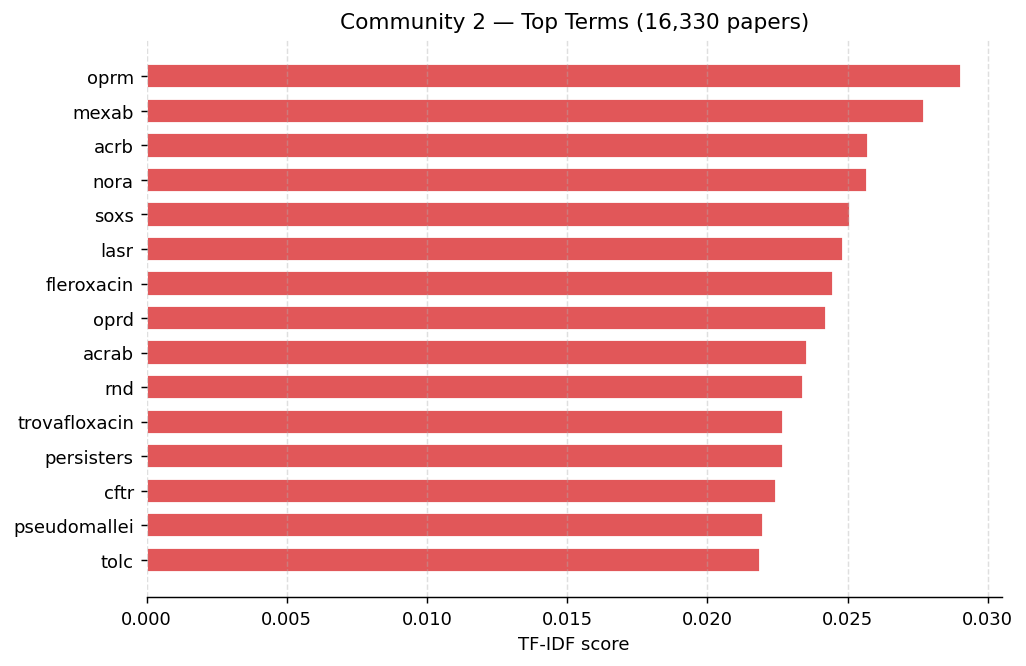
\includegraphics[width=\textwidth]{top_terms_c2.png}
        \caption{Top TF-IDF terms for Community C2 (Efflux pumps / Gram-negatives).}
    \end{subfigure}
    \caption{Horizontal bar charts of TF-IDF scores for the two largest communities.
             Higher scores indicate terms that are more distinctive for that community
             relative to all others.}
    \label{fig:tfidf}
\end{figure}

\subsubsection{Other Major Communities}

The remaining large communities are equally well-defined:

\begin{itemize}
    \item \textbf{C102 -- Plasmid genetics and horizontal gene transfer.}
    Top papers include foundational molecular biology work such as
    \textit{``Colicinogeny and related phenomena''} (1976, degree 545) and
    \textit{``The pUC plasmids''} (1983, degree 493).
    This community was dominant in the 1970s and 1980s, when the genetic basis of
    resistance transfer was being characterised for the first time.

    \item \textbf{C4 -- Gram-positive pathogens (MRSA and VRE).}
    Centred on \textit{Staphylococcus aureus} and \textit{Enterococcus}, with top
    papers on the genetic basis of methicillin and glycopeptide resistance.

    \item \textbf{C36 -- Mycobacterium tuberculosis.}
    The highest-degree paper is the TB genome paper (1998, degree 346), and the top MeSH
    descriptors include Mycobacterium tuberculosis, antitubercular agents, and molecular
    epidemiology.

    \item \textbf{C10 -- HIV antiviral resistance.}
    A reminder that AMR as defined by the MeSH vocabulary encompasses antiviral as well
    as antibacterial resistance.

    \item \textbf{C37 -- Antifungal resistance.}
    Covering \textit{Candida} and \textit{Aspergillus} species, with papers on azole and
    polyene resistance mechanisms.
\end{itemize}

\subsection{Temporal Evolution}

\subsubsection{Community Growth}

Figure~\ref{fig:growth} shows the number of new publications per 5-year window for the
ten largest communities.

\begin{figure}[H]
    \centering
    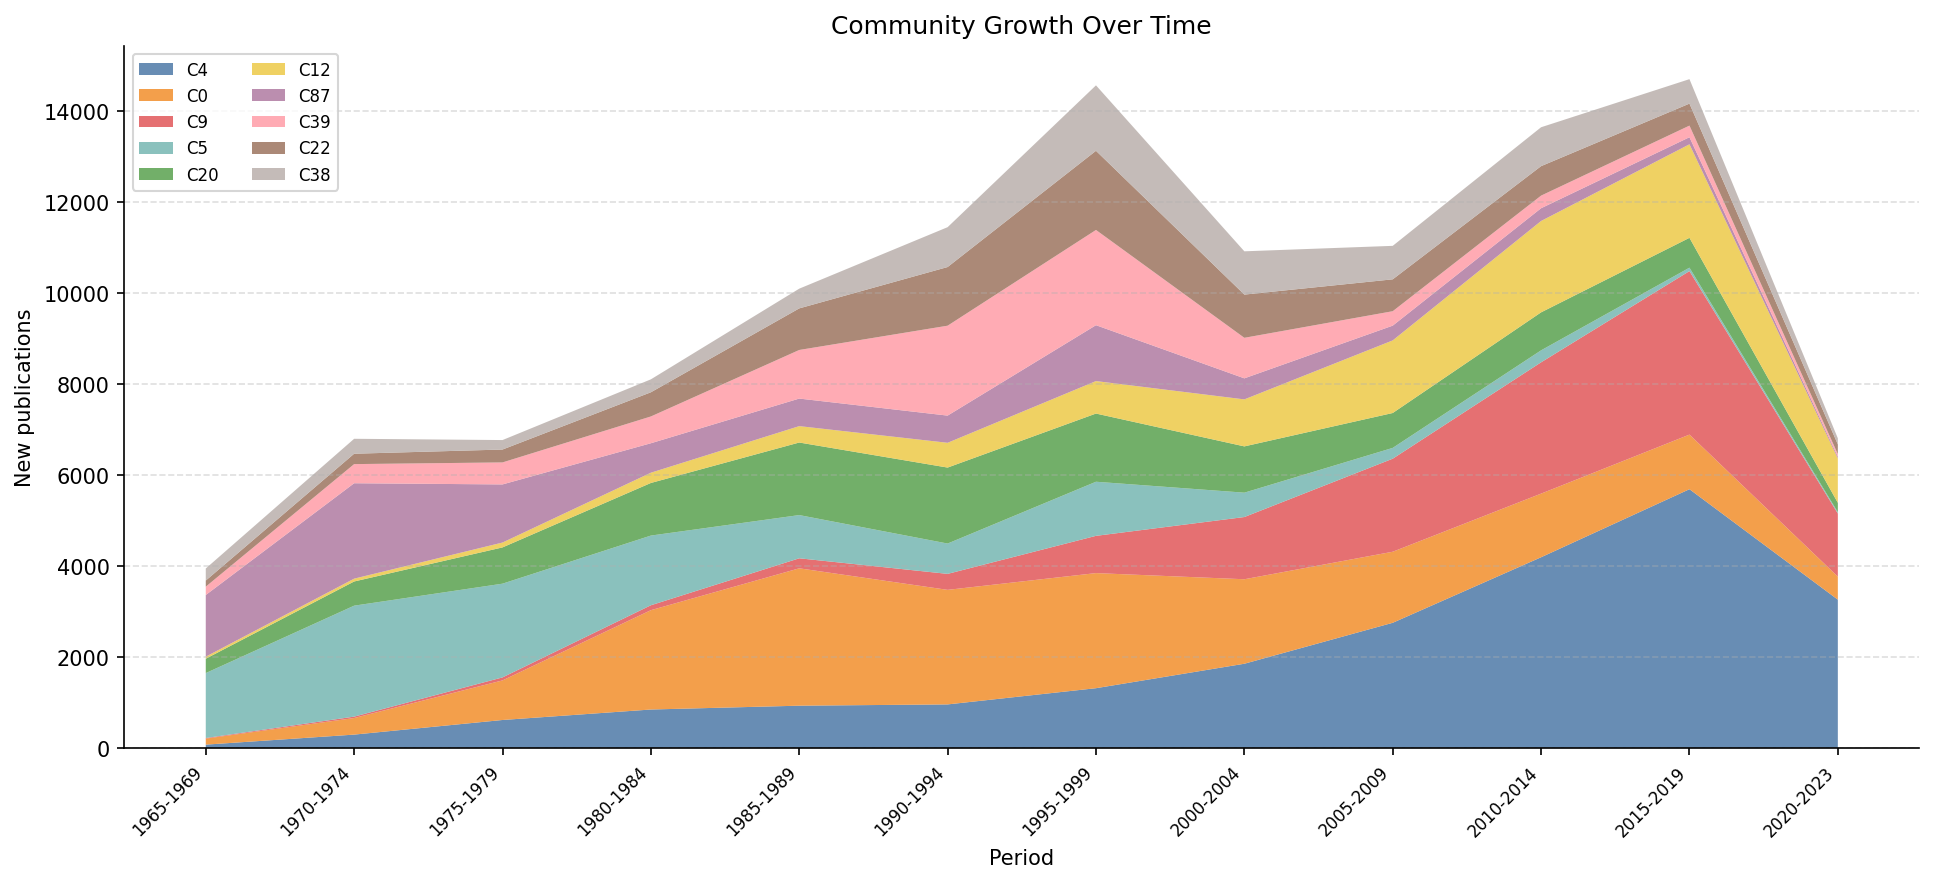
\includegraphics[width=\textwidth]{community_growth.png}
    \caption{Stacked area chart of new publications per 5-year period for the ten
             largest communities. The 2020--2023 window covers only four years.}
    \label{fig:growth}
\end{figure}

Several patterns stand out:

\begin{itemize}
    \item \textbf{C102 dominates early periods (1965--1984).} This is consistent with
    the historical record: the 1970s and early 1980s were the golden era of plasmid
    biology and molecular genetics, when the mechanisms of resistance transfer were
    being established.

    \item \textbf{A dip around 2000--2004} is visible across most communities.
    This corresponds to a well-documented withdrawal of major pharmaceutical companies
    from antibiotic R\&D during the late 1990s and early 2000s, driven by economic
    factors and the perceived difficulty of the antibiotic discovery problem.

    \item \textbf{C65 (environmental AMR) is barely visible before 2005 and then
    explodes.} This matches the policy timeline: the 2006 EU ban on antibiotic growth
    promoters in livestock, followed by the 2015 WHO Global Action Plan on AMR, triggered
    an enormous surge in One Health and environmental AMR research.

    \item \textbf{The overall upward trend from 2005 to 2019} reflects the growing global
    recognition of AMR as a public health emergency and the increased research funding
    that followed.

    \item \textbf{The 2020--2023 window} shows a drop in total publications relative to
    2015--2019. This is partly a methodological artefact: the window covers only four
    years, not five, and very recent papers have had less time to accumulate citations
    within the dataset.
\end{itemize}

\subsubsection{Centrality Evolution}

Figure~\ref{fig:degree_evol} shows the average degree per community in each 5-year window.
This metric captures how densely connected papers within a community were \textit{at that
time}, i.e., how many other papers published in the same period they cited or were cited by.

\begin{figure}[H]
    \centering
    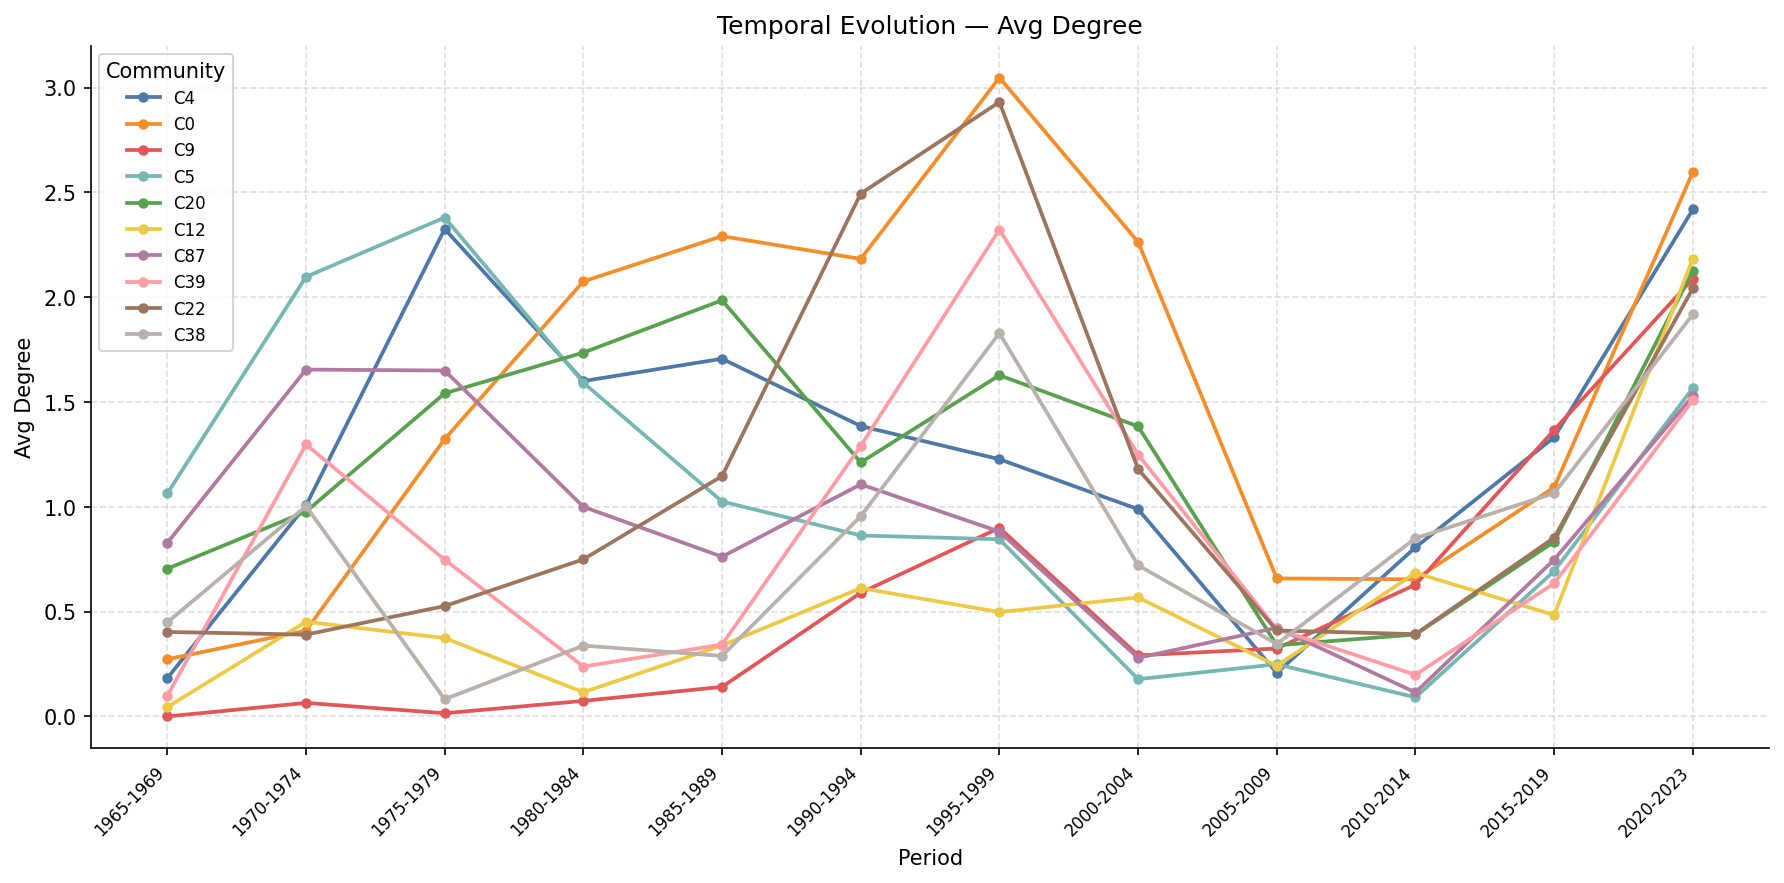
\includegraphics[width=\textwidth]{centrality_evolution_avg_degree.png}
    \caption{Average degree per community per 5-year window.
             Higher values indicate denser internal citation activity in that period.}
    \label{fig:degree_evol}
\end{figure}

Key observations:

\begin{itemize}
    \item \textbf{C102} (plasmid genetics) has the highest average degree in the early
    windows (1970--1979), reaching 2.4 in 1975--1979.
    This reflects a highly interconnected body of foundational genetics papers that
    cited each other extensively.

    \item \textbf{C2} (efflux pumps) peaks in 1995--1999 at 3.1, the highest value
    of any community in any period.
    This corresponds precisely to the years when RND-type efflux systems were
    characterised in \textit{P. aeruginosa} and \textit{E. coli}, producing a burst of
    closely cross-cited papers \cite{nikaido2009}.

    \item \textbf{C65} (environmental AMR) shows low degree until 2010 and then rises
    sharply, reaching 2.86 in 2020--2023 --- the highest value of any community in the
    most recent period.
    This means that environmental AMR papers published between 2020 and 2023 are
    intensely cross-citing each other, indicating a very active and cohesive research
    front.

    \item The general pattern of a \textbf{valley around 2005--2009} followed by a
    rise is consistent across most communities and corroborates the narrative of a
    post-2000 slowdown followed by renewed activity.

    \item The \textbf{inverted-U shape} observed in most communities is a methodological
    feature of windowed citation analysis: papers from 25 years ago have had much more
    time to accumulate mutual citations within their window than papers published last
    year.
    This should be kept in mind when comparing absolute degree values across periods.
\end{itemize}

\subsection{Most Influential Papers}

Table~\ref{tab:top_papers} lists the most connected paper (by total degree) in each of
the five largest communities.

\begin{table}[H]
\centering
\caption{Most connected paper (highest degree) in each of the five largest communities.}
\begin{tabular}{p{0.5cm}rp{8cm}r}
\toprule
\textbf{Comm.} & \textbf{Year} & \textbf{Title} & \textbf{Degree} \\
\midrule
C65  & 2022 & Evolutionary Pathways and Trajectories in Antibiotic Resistance & 617 \\
C8   & 2014 & Antibiotic resistance -- the need for global solutions              & 335 \\
C2   & 2015 & The challenge of efflux-mediated antibiotic resistance in Gram-negative bacteria & 1\,176 \\
C102 & 1976 & Colicinogeny and related phenomena                                  & 545 \\
C37  & 1998 & Clinical, cellular, and molecular factors that contribute to antifungal drug resistance & 292 \\
\bottomrule
\end{tabular}
\label{tab:top_papers}
\end{table}

The paper in C2 stands out with a degree of 1\,176, making it the single most structurally
important paper in the entire network.
Its high connectivity reflects the central role of efflux mechanisms as a unifying theme
across \textit{P. aeruginosa}, \textit{E. coli}, and many other Gram-negative pathogens
studied in the AMR literature.

% ============================================================
\section{Discussion}

\subsection{Quality of the Community Structure}

The modularity value of 0.746 is high by any standard (values above 0.3 are generally
considered non-trivial \cite{fortunato2010}).
This suggests that the citation network has genuine modular structure and is not simply a
random graph.
The biological interpretability of the communities -- each corresponding to a well-known
research field -- further validates this.

The fact that the four largest communities each contain 15\,000--18\,000 papers, and
are roughly equal in size, is itself an interesting observation.
It suggests that AMR research is not dominated by a single paradigm but is genuinely
multi-disciplinary, with equally prominent communities addressing molecular mechanisms,
environmental spread, clinical resistance, and genetic transfer.

\subsection{TF-IDF as a Topic Label}

The TF-IDF approach works well for this corpus because AMR sub-fields have very
different vocabularies.
Efflux pump researchers write about \textit{mexAB}, \textit{acrB}, and \textit{RND};
environmental researchers write about \textit{wwtps}, \textit{composting}, and
\textit{ARGs}; tuberculosis researchers write about \textit{isoniazid} and
\textit{rifampicin}.
These distinctive vocabularies produce high TF-IDF scores for informative terms and
allow automatic labelling with high confidence.

\subsection{Limitations}

Several limitations should be noted.
First, the windowed temporal analysis produces lower average degree values for recent
periods simply because recent papers have had less time to accumulate citations.
This makes direct comparison of degree values across time periods misleading without
normalisation.
Second, the betweenness centrality was approximated by vertex sampling for computational
reasons; exact betweenness on a graph of this size would take several hours.
Third, the \texttt{on\_topic = False} papers are structurally important (they provide
the backbone of the citation network) but are not directly retrieved for AMR content,
which means some community labels may be influenced by foundational papers from adjacent
fields.

% ============================================================
\section{Conclusion}

This project demonstrates that citation network analysis combined with text mining is
an effective approach for automatically mapping the structure of a large scientific
literature.
Applied to the AMR field, the methodology identifies biologically coherent communities,
labels them with distinctive vocabulary, and tracks their evolution over six decades.

The key findings are:
\begin{enumerate}
    \item The AMR citation network has strong community structure (modularity 0.746)
          with roughly four equally dominant research pillars.
    \item Environmental AMR and the One Health framework have grown from a marginal
          topic to the most actively cited community in 2020--2023, reflecting the
          post-2015 policy push triggered by the WHO Global Action Plan.
    \item The foundational plasmid genetics community (C102) dominated the early
          literature (1970s--1980s) and has been gradually superseded by communities
          addressing contemporary clinical and environmental challenges.
    \item TF-IDF analysis on community-level text aggregates reliably recovers the
          specialised vocabulary of each sub-field, enabling automatic topic labelling.
    \item The most structurally important paper in the network is a 2015 review on
          efflux-mediated resistance in Gram-negative bacteria, with a degree of 1\,176.
\end{enumerate}

Future work could extend this analysis to co-authorship networks and keyword co-occurrence
networks to obtain a complementary view of the field's structure,
or apply the framework to track the impact of specific WHO priority pathogens over time.

% ============================================================
\newpage
\bibliographystyle{unsrtnat}
\begin{thebibliography}{99}

\bibitem{who_amr_2015}
World Health Organization.
\newblock {Global Action Plan on Antimicrobial Resistance}.
\newblock Technical report, WHO, Geneva, 2015.
\newblock \url{https://www.who.int/publications/i/item/9789241509763}

\bibitem{blondel2008}
V.~D. Blondel, J.-L. Guillaume, R.~Lambiotte, and E.~Lefebvre.
\newblock Fast unfolding of communities in large networks.
\newblock \textit{Journal of Statistical Mechanics: Theory and Experiment},
  2008(10):P10008, 2008.

\bibitem{newman2006}
M.~E.~J. Newman.
\newblock Finding community structure in networks using the eigenvectors of
  matrices.
\newblock \textit{Physical Review E}, 74(3):036104, 2006.

\bibitem{fortunato2010}
S.~Fortunato.
\newblock Community detection in graphs.
\newblock \textit{Physics Reports}, 486(3--5):75--174, 2010.

\bibitem{igraph2006}
G.~Cs{\'a}rdi and T.~Nepusz.
\newblock The igraph software package for complex network research.
\newblock \textit{InterJournal, Complex Systems}, 1695(5):1--9, 2006.

\bibitem{salton1988}
G.~Salton and C.~Buckley.
\newblock Term-weighting approaches in automatic text retrieval.
\newblock \textit{Information Processing \& Management}, 24(5):513--523, 1988.

\bibitem{blair2015}
J.~M.~A. Blair, M.~A. Webber, A.~J. Baylay, D.~B. Ogbolu, and L.~J.~V. Piddock.
\newblock Molecular mechanisms of antibiotic resistance.
\newblock \textit{Nature Reviews Microbiology}, 13(1):42--51, 2015.

\bibitem{nikaido2009}
H.~Nikaido.
\newblock Multidrug resistance in bacteria.
\newblock \textit{Annual Review of Biochemistry}, 78:119--146, 2009.

\bibitem{onehealth}
T.~P. Van~Boeckel, C.~Brower, M.~Gilbert, B.~T. Grenfell, S.~A. Levin,
  T.~P. Robinson, A.~Teillant, and R.~Laxminarayan.
\newblock Global trends in antimicrobial use in food animals.
\newblock \textit{Proceedings of the National Academy of Sciences},
  112(18):5649--5654, 2015.

\bibitem{martin2011}
S.~Martin, W.~M. Brown, R.~Klavans, and K.~W. Boyack.
\newblock {OpenOrd}: An open-source toolbox for large graph layout.
\newblock In \textit{Proceedings of SPIE -- Visualization and Data Analysis},
  volume 7868, 2011.

\end{thebibliography}

\end{document}
